\newcommand{\assignmentDate}{November 11th, 2019}

% Add title
%Institute
\begin{tabular*}{\hsize}{l@{\extracolsep{\fill}} r}
	\textsc{Technical University of Berlin}		 \hfill&								 	\\
	Faculty II - Mathematics and Natural Sciences\hfill&									\\
	Institute of Mathematics 					 \hfill&									\\
	Dr. D. Peschka, A. Selahi 		 			 \hfill&									\\
\end{tabular*}

% Title
\begin{center}
	\textbf{\Large{\courseName}}\\
	\vspace{7pt}
	\large{Homework \currentAssignment}\\
	\smallskip
	\normalsize{Submitted on \assignmentDate}
\end{center}

% Group table
\begin{center}
	\vspace{-8pt}
	\begin{tabular}{l c r}
		by \textbf{\groupNumber}		    &	 			  &		 								\\
		\hline
		\texttt{Kagan Atci} 			    & \texttt{338131} & \texttt{Physical Engineering, M.Sc.}\\
		\texttt{Navneet Singh }		 	    & \texttt{380443} & \texttt{Scientific Computing, M.Sc.}\\ 
		\texttt{Daniel V. Herrmannsdoerfer} & \texttt{412543} & \texttt{Scientific Computing, M.Sc.}\\ 
		\hline
	\end{tabular}
\end{center}

% EXERCISE 1
% --------------------------------------------------------------------------------------------------------------------
\newcommand{\Sk}{\MAT{S}}
\addExercise{1}{Ex1}
Given is $m \in \mathbb{N}_0$, assuming $\bar{\Omega} = [0,1]$ and $\bar{\Omega}_h = \{0,h,\dots,(N+1)h\}$ with $h = \frac{1}{N + 1}$ the corresponding grid.
Considering that $x_n = nh \in \bar{\Omega}_h$ with sufficiently many neighbors to either side, for any $j$ with $n-m \leq j \leq n+m$, requiring $x_j = jh \in \bar{\Omega}_h $, and $u_n = u(x_n)$ with $u \colon \bar{\Omega} \rightarrow \mathbb{R}$ is $r$ times continuously differentiable.

%
% ----------------
\addSubExercise{a}
$u$ values on neighbor points with above mentioned conditions are expressed in Taylor expansion form about the $x_n$
\begin{align}
	u_h(x_n + j h) = u_h(x_n) + u^\prime(x_n)\frac{(jh)^1}{1!} + u_h^{\prime\prime}\frac{(jh)^2}{2!} + \cdots + u_h(x_n) \frac{(jh)^k}{k!} + R
\end{align}
with $k$ the derivative order and $R$ the remainder.
Applying this for each neighbor point, a linear equation system between the $u$ and their derivatives is built up
\begin{equation}
	\BMAT{u_h(x_{n-m})     \\
		  \vdots 		   \\
		  u_h(x_{n+ m})}
	= \Sk \;
	\BMAT{u(x_n)     \\
		  \vdots 		   \\
		  h^{k}u^{(k)}(x_n)}
	\text{ where } \Sk \in \mathbb{R}^{k \times k} \text{ with } s_{j,k} = \frac{j^k}{k!} \text{.}
\end{equation}
In this case, the symmetric stencils for spatial differentiations $\Delta_{h,r}$ up to $k$-th order are obtained by inverting $\Sk$, where the remainders are neglected.
\begin{equation}
	\Sk^-1 \;
	\BMAT{u_h(x_{n-m})     \\
		  \vdots 		   \\
		  u_h(x_{n+ m})}
	=
	\BMAT{u(x_n)     \\
		  \vdots 		   \\
		  h^{k}u^{(k)}(x_n)}
\end{equation}
Since the $\Sk^{-1}$ must be a symmetric matrix, applying the Taylor expansion procedure to $m$ neighbor points on either sides limits the derivative order at $k=2m + 1$ for $u$ being $r=2m + 2$ differentiable.
Hence, the remainder can also be written in the matrix form as
\begin{equation}
	\MAT{R} \in \mathbb{R}^{k \times k} \text{ with } r_{j,k} = \frac{(jh)^{r}}{r!}u^{(r)}(\xi)$ \text{ for } $\xi \in [x_n -kh, x_n + kh]\text{.}
\end{equation}

%
% ----------------
\addSubExercise{b} Please refer to online submitted \texttt{a03ex01getstencil.m} file.

%
% ----------------
\addSubExercise{c} Please refer to online submitted \texttt{a03ex01getLaplace.m} file.

%
% ----------------
\addSubExercise{d}
For $u(x) = \sin{(2\pi x)}, $\text{ }\FIG{a03e01DiffError} illustrates the maximum error magnitude between the finite difference method with four different level of stencils and the analytical method applied on $u^{\prime\prime}$.
\begin{figure}[H]
\vspace*{\FigUpperVSpace}
	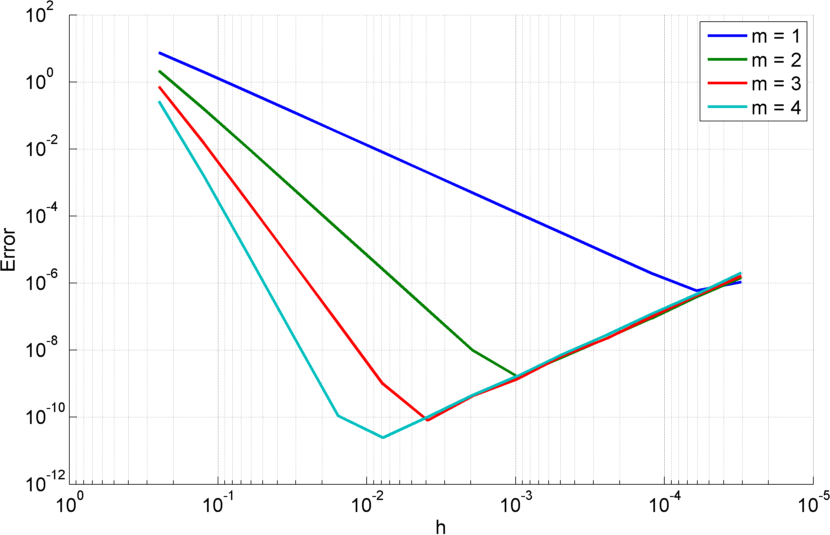
\includegraphics[width=\textwidth]{a03e01DiffError.png} 
	\caption{Maximum error $\max_j|L_h(x_j)u_h(x_j)-u^{\prime\prime}(x_j)|$ of the finite difference stencils as a function of $h$ with respect to $m$}
	\label{fig:a03e01DiffError}
\end{figure}
Accordingly, a straight conclusion regarding to an exponential error reduction by increasing the mesh resolution (deceasing $h$) can be made in the first place.
This is also considered as an improvement in convergence.
Furthermore, increasing the number of neighbor points in constructing the finite difference stencil leads to the improvement of convergence at even higher rates.
However, the error, which in theory is supposed to go to 0 continuously for $\lim_{h\rightarrow0}$, stops this behavior at a certain $h$ for every $m$.
This is issue is associated with the rounding error of the computer.
The more neighbor points are used for the stencil, the sooner can this limit be reached.
Therefore, this limiting fact must be taken into account during geometry meshing.

% EXERCISE 2
% --------------------------------------------------------------------------------------------------------------------
\addExercise{2}{Ex2}
%
% ----------------
\addSubExercise{a, b \& c} See the handwritten solutions.

% EXERCISE 3
% --------------------------------------------------------------------------------------------------------------------
\addExercise{3}{Ex3}
Considered is the boundary value problem (BVP)
\begin{equation}
	\begin{cases}
		-u^{\prime\prime}(x) - 4u^\prime(x) + u(x) = f(x), \text{ for all } x \in \Omega = (0,1) \\
		u(0)=1, u(1) = 2 \text{ .}
	\end{cases}
\end{equation}

%
% ----------------
\addSubExercise{a}
Assuming that the exact solution is $1 + 4x^2 - 3x^3$, the analytical solution of the BVP's right hand side is
\begin{equation}
	f(x) = -3x^3 + 40x^2 - 14x -7
\end{equation}

%
% ----------------
\addSubExercise{b}
Please refer to online submitted \texttt{a03ex03getBVP.m} file.

%
% ----------------
\addSubExercise{c}
For the programming solution, please refer to online submitted \texttt{a03ex03solve.m} file.
The error between the approximation and the restricted exact solution is illustrated in \FIG{a03ex03error} in the form of maximum norm.
Accordingly, $error(p)$ goes with a near constant exponential rate towards 0, as $h \rightarrow 0$.
\begin{figure}[H]
	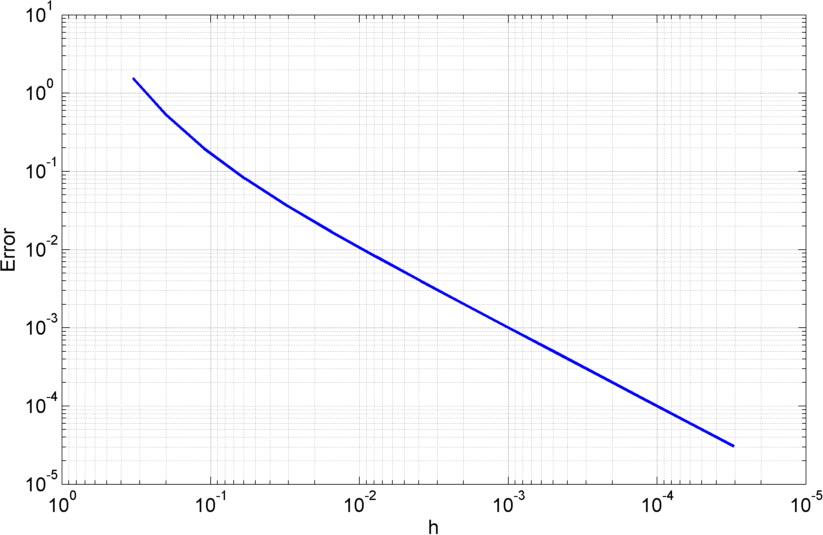
\includegraphics[width=\textwidth]{a03ex03error.png} 
	\caption{Maximum error $\max_i|u_h (ih)-u(ih)|$ between the approximation and the exact solution}
	\label{fig:a03ex03error}
\end{figure}